\subsection*{Problema 09}
\textbf{Enunciado:} Calcular la integral:
\begin{align*}
\int \sqrt{x^2 + x + 1} \, dx
\end{align*}

\textbf{Solución:} Primero completamos el cuadrado en el radicando:
\begin{align*}
x^2 + x + 1 &= \left(x^2 + x + \dfrac{1}{4}\right) + 1 - \dfrac{1}{4} \\
&= \left(x + \dfrac{1}{2}\right)^2 + \dfrac{3}{4}
\end{align*}

Sustituyendo esto en la integral, obtenemos:
\begin{align*}
\int \sqrt{\left(x + \dfrac{1}{2}\right)^2 + \dfrac{3}{4}} \, dx
\end{align*}

Utilizamos la sustitución trigonométrica:
\begin{align*}
x + \dfrac{1}{2} &= \dfrac{\sqrt{3}}{2} \tan\theta \\
dx &= \dfrac{\sqrt{3}}{2} \sec^2\theta \, d\theta
\end{align*}

El radicando se transforma en:
\begin{align*}
\sqrt{\left(\dfrac{\sqrt{3}}{2}\tan\theta\right)^2 + \dfrac{3}{4}} &= \sqrt{\dfrac{3}{4}(\tan^2\theta + 1)} \\
&= \dfrac{\sqrt{3}}{2} \sec\theta
\end{align*}

Sustituyendo $dx$ y el radical:
\begin{align*}
&= \int \left(\dfrac{\sqrt{3}}{2} \sec\theta\right) \left(\dfrac{\sqrt{3}}{2} \sec^2\theta \, d\theta\right) \\
&= \dfrac{3}{4} \int \sec^3\theta \, d\theta
\end{align*}

Usando la integral conocida de $\sec^3\theta$:
\begin{align*}
&= \dfrac{3}{8} \left( \sec\theta \tan\theta + \ln|\sec\theta + \tan\theta| \right) + C
\end{align*}

Regresando a la variable original $x$:
\begin{align*}
\tan\theta &= \dfrac{2x + 1}{\sqrt{3}}, \quad \sec\theta = \dfrac{2\sqrt{x^2 + x + 1}}{\sqrt{3}}
\end{align*}

Sustituyendo y simplificando, el resultado final es:
\begin{align*}
\int &\sqrt{x^2 + x + 1} \, dx = \dfrac{2x + 1}{4} \sqrt{x^2 + x + 1} \\
&+ \dfrac{3}{8} \ln\left| \dfrac{2\sqrt{x^2 + x + 1} + 2x + 1}{\sqrt{3}} \right| + C
\end{align*}

\begin{figure}[H]
	\centering
	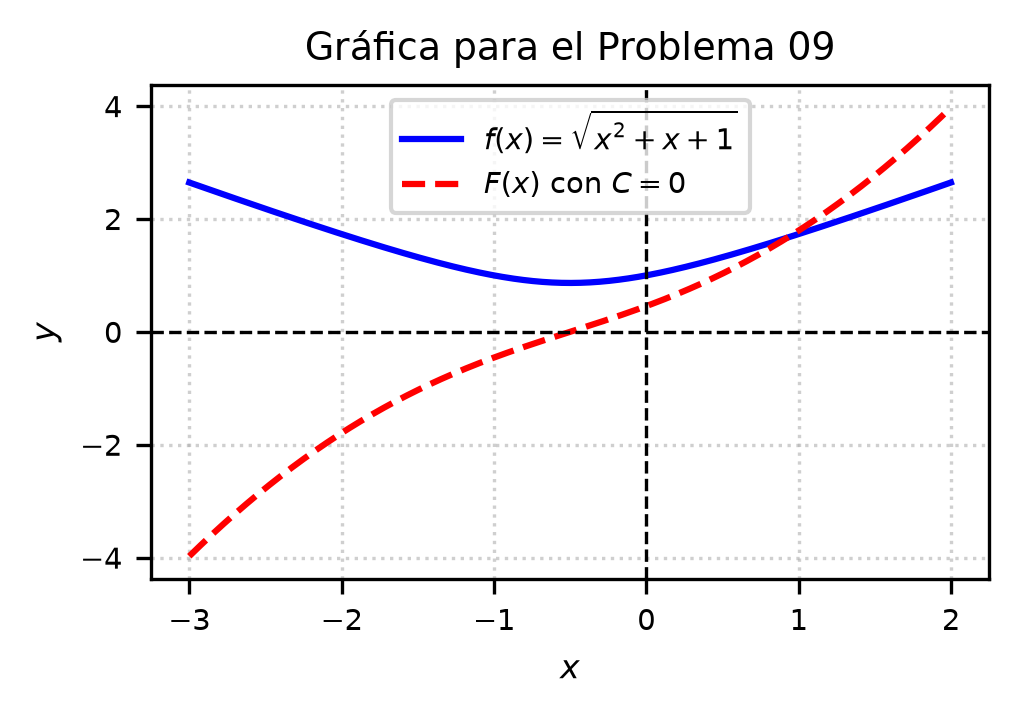
\includegraphics[width=\columnwidth]{semana_05/graficas/SEM05_P09_grafica.png}
	\caption{Representación gráfica de $f(x)$ y su antiderivada $F(x)$ evaluada para la constante de integración $C = 0$ (Problema 09).}
	\label{fig:problema09}
\end{figure}
